\section{Prepogibanje stožnic}
\label{pogl:stoznice}

% kako konstruiramo tangente na stožnice in zakaj konstrukcije tako delujejo
% parabola, elipsa, hiperbola
% povezava z O6
% pa omeni tudi O7, kjer je skupna tangenta na dve paraboli
% a za krožnico se tudi da?

Iz didaktičnega vidika zelo zanimivo poglavje nam predstavlja konstrukcije tangent na stožnice s prepogibanjem papirja. Vsebina je tu predstavljena tako, da je bralec najprej povabljen, da vzame list papirja in ga prepogiba po navedenih korakih. Po opažanju, kaj se na papirju pri tem prikaže, preidemo na matematični del, kjer dokažemo, da so prepogibi res tangente na določeno stožnico.

Učitelji matematike so povabljeni, da si pri obravnavi stožnic vzamejo čas in izvedejo spodnje aktivnosti. Dijaki bodo z veliko verjetnostjo presenečeni nad rezultati zgibanja, kar jih lahko bolj motivira za obravnavo geometričnih lastnosti stožnic. Priporočljiva je tudi izvedba ure v računalniški učilnici, kjer lahko vsak dijak z ustreznim programskim orodjem (npr.\ Geogebra) sam poskusi zgraditi opisano konstrukcijo. S tem lahko znanje o stožnicah le še bolj utrdi.

\subsection{Parabola}

\textit{\textbf{Aktivnost:} Vzemi pravokoten list papirja in svinčnik ter nekje sredi spodnje polovice lista s pisalom označi točko. Nato si izberi točko še na spodnji stranici lista in ga prepogni tako, da se obe izbrani točki prekrijeta. To ponovi čimvečkrat (gl.\ sliko~\ref{fig:koraki_parabola}). Kaj opaziš?}

\begin{figure}[h]
    \centering
    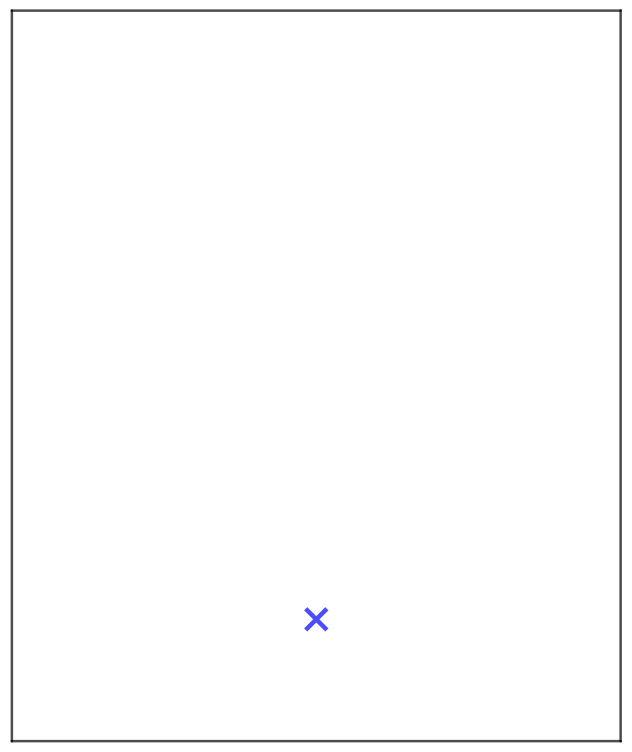
\includegraphics[width=0.3\textwidth]{images/stožnice/folding_parabola_1.png}
    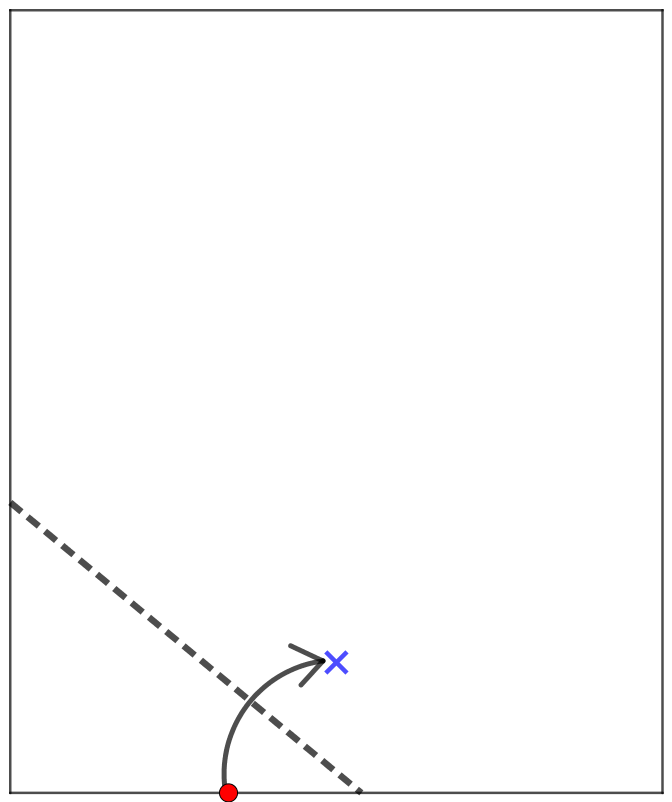
\includegraphics[width=0.3\textwidth]{images/stožnice/folding_parabola_2.png}
    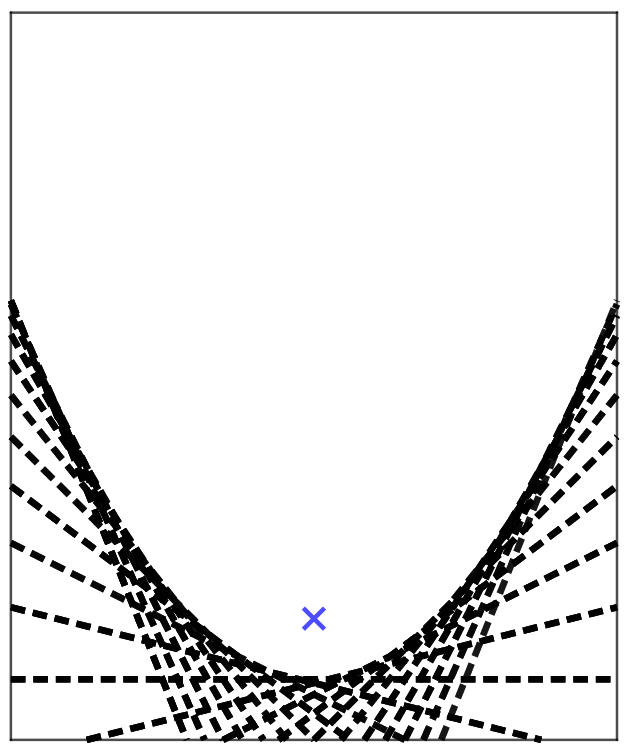
\includegraphics[width=0.3\textwidth]{images/stožnice/folding_parabola_3.png}
    \caption[Prepogibanje parabole]{Prepogibanje spodnje stranice papirja na izbrano točko.}
    \label{fig:koraki_parabola}
\end{figure}

% Najstareši opis zgornje konstrukcije, ker sem jih našla, je v svojo knjigo \emph{Geometric Exercises in Paper Folding} vključil indijski matematik T.\ Sundara Row~\cite{row1917}.
% Hull je našel Row-a (prvič izdana 1893) kot najstarejši zapis te konstrukcije

Omenjen pregib je origami operacija~\ref{op:O3}, lahko pa nanjo gledamo tudi kot na operacijo~\ref{op:O6}. Za le-to smo v poglavju~\ref{pogl:aksiomi} že premislili, da nam pregib, ki poteka skozi dano točko $B$ in točko $A$ položi na premica $a$, poda tangento na parabolo z goriščem $A$ in premico vodnico $a$ (gl.\ sliko~\ref{fig:O6_parabola} in premislek nad njo). Tukaj pa take točke $B$ ni, kar pomeni le to, da smo s pregibom konstruirali neko tangento -- pregib je namreč simetrala daljice, ki ima za krajišči obe izbrani točki iz navodil naloge, torej obstaja točka (točka $P$ na sliki~\ref{fig:O6_parabola}), ki je enako oddaljena od spodnje stranice lista in prve izbrane točke. Nadaljni premislek, da je to edino presečišče pregiba in parabole, je enak kot prej.

Po večkrat izvedenih pregibih spodnje stranice lista na začetno izbrano točko dobimo na papirju obris krivulje. Ker so pregibi tangente na parabolo, predvidevamo, da je ta krivulja ravno parabola. Vendar moramo to dokazati. V ta namen si -- brez škode za splošnost, saj lahko z origamijem zrcalimo in rotiramo točke ter premice -- model poljubne točke in  spodnje stranice lista natančno določimo. Uporabimo že znan model iz dokaza izreka~\ref{izr:origami_konstruktibilnost} (pri konstrukciji $\sqrt{r}$): vzemimo točko $A(0, 1)$ in premico $a: y = -1$, ki sta origami-konstruktibilni, in naredimo pregib, ki točko $A$ preslika na premico $a$ v točko $A'(t, -1)$ za nek $t \in \R$ (slika~\ref{fig:enacba_tangente_par1}).

\begin{figure}[h]
    \centering
    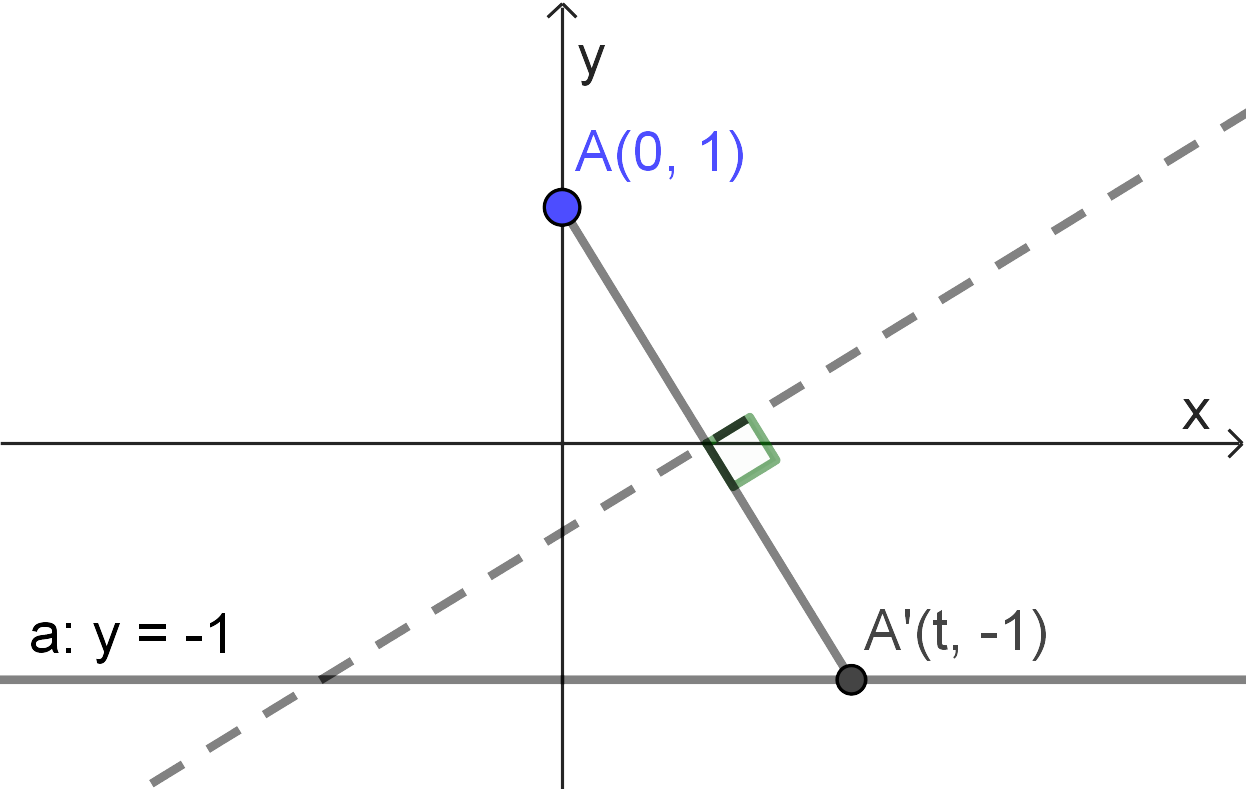
\includegraphics[width=0.5\textwidth]{images/enacba_parabole1.png}
    \caption[Enačba tangente na parabolo]{Pregib točke $A(0, 1)$ na premico $a: y = -1$.}
    \label{fig:enacba_tangente_par1}
\end{figure}

Ker je pregib oz.\ konstruirana premica simetrala daljice $AA'$, lahko hitro določimo njeno enačbo. Koeficient nosilke daljice $AA'$ je $k_A = -\frac{2}{t}$, središče pa $(\frac{t}{2}, 0)$. Tako hitro določimo enačbo pregiba:
\begin{equation}
    y = \frac{t}{2} x - \frac{t^2}{4}.
    \label{eq:tang_par}
\end{equation}
Dobili smo parametrizacijo neke družine premic. Za vsak $t \in \R$ torej dobimo drugo tangento na parabolo z goriščem v točki $A$ in premico vodnico $a$, ki ima zgornjo enačbo.

Za vse točke na pregibu velja, da so enako oddaljene od točk $A$ in $A'$. Vemo že, da obstaja le ena točka $T \in a$, za katero velja $d(T, A) = d(T, a)$. Njena abscisa je $x = t$ (točka $T$ leži na pregibu točno nad točko $A'$) in iz enačbe~\ref{eq:tang_par}, dobimo še ordinato $y = t^2 / 4$. Ker točka $T$ za vsak $t \in \R$ leži na paraboli, pri menjavi $x = t$ dobimo njeno enačbo: $y = x^2 / 4$.

Vendar to ni dokaz, da je obris pregibov iz naloge res parabola. Zgornji premislek temelji na že znanem dejstvu, da so pregibi tangentni na parabole, vendar nam nič ne zagotavlja, da take točke $T$ ležijo točno na obrisu.

Hull v~\cite[str.\ 55--56]{hull2013} poda prefinjen dokaz preko kvadratne formule. Vemo, da pregib~\ref{op:O6} ne obstaja vedno (slika~\ref{fig:O6} desno). Poglejmo, ali obstajajo v ravnini našega modela kakšne točke, skozi katere ne moremo konstruirati pregiba oz.\ tangente. Vzemimo našo parametrizacijo družine tangent (enačba~\ref{eq:tang_par}). Če jo rešimo za $t$, nam dobljena formula pove, za katere vrednosti $t$ pregib poteka skozi točko $(x, y)$:
$$ \frac{1}{4}t^2 - \frac{x}{2}t + y = 0 \Rightarrow t_{1,2} = \frac{\frac{x}{2} \pm \sqrt{\frac{x^2}{4} - y}}{\frac{1}{2}}.$$
Enačba ima dve realni rešitvi pri pogoju $x^2 / 4 - y > 0$, kar pomeni, da vsako točko $(x, y)$, za katero ta pogoj velja, sekata dva pregiba. To so ravno točke pod parabolo $y = x^2 / 4$. Za točke \emph{na} paraboli velja $y = x^2 / 4$, iz česar dobimo eno rešitev $t = x$, torej to točko seka natanko en pregib. Nazadnje nam ostane še območje, za katerega velja $y > x^2 / 4$, t.\ j.\ območje nad parabolo $y = x^2 / 4$, kar nam ne poda realnih rešitev za $t$, torej ga ne seka noben izmed konstruiranih pregibov. Tako je obris, ki ga dobimo v nalogi, res parabola $y = x^2 / 4$.

Torej je naš razmislek dva odstavka višje utemeljen. Sedaj, ko vemo, da je obris, ki nastane po večkratnem prepogibu spodnje stranice lista papirja na izbrano točko, res parabola, lahko pogledamo še več načinov za določitev enačbe parabole~\cite[str.\ 55--56]{hull2013}:
\begin{itemize}
    \item Naj bo $y(x)$ naša parabola, katere enačbo iščemo. Vemo, da je v našem modelu za poljuben $t \in \R$ pregib v neki točki $(x, y(x))$ tangenten na parabolo, koeficient tangente pa je $t / 2$. Očitno velja $x = t$, torej je koeficient kar $x / 2$. Zato dobimo
    $$ \frac{dy}{dx} = \frac{x}{2} \Rightarrow y = \frac{x^2}{4} + C. $$
    Ker parabola očitno poteka skozi točko $(0, 0)$, je $C = 0$ in dobimo želeno enačbo $y = x^2 / 4$.
    \item \textcolor{red}{Envelope way -- gl.\ ~\cite[str.\ 56 spodaj]{hull2013} (tema iz diferencialne ali algebraične geometrije).}
\end{itemize}

\textcolor{red}{na koncu še O7 -- konstrukcija skupne parabole na dve paraboli -- a se da iz tega še kaj pametnega izcimit?}

Aktivnosti za naslednji dve podpoglavji sta enaki kot v tem, le da namesto spodnje tranice lista v izbrano točko prepogibamo krožnico.

\subsection{Elipsa}

\textit{\textbf{Aktivnost:} Vzemi list papirja in svinčnik ter na sredini nariši poljubno krožnico. Označi njeno središče. Na notranji strani krožnice si izberi poljubno točko. Izberi si točko na krožnici in list prepogni tako, da se obe izbrani točki prekrijeta. To ponovi čimvečkrat (gl.\ sliko~\ref{fig:koraki_elipsa}). Kaj opaziš?}

\begin{figure}[h]
    \centering
    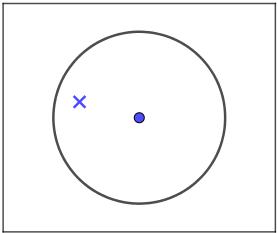
\includegraphics[width=0.3\textwidth]{images/stožnice/folding_elipsa_1.png}
    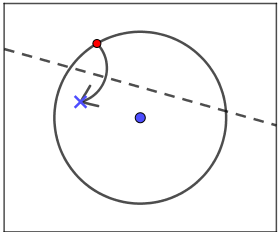
\includegraphics[width=0.3\textwidth]{images/stožnice/folding_elipsa_2.png}
    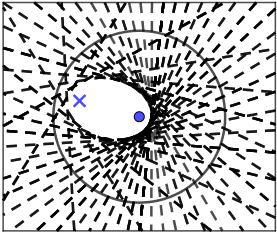
\includegraphics[width=0.3\textwidth]{images/stožnice/folding_elipsa_3.png}
    \caption[Prepogibanje elipse]{Prepogibanje krožnice na izbrano točko znotraj nje.}
    \label{fig:koraki_elipsa}
\end{figure}

\opomba{Za izris poljubne krožnice tu lahko uporabimo šestilo. Se je pa mogoče uporabi drugih orodij tudi izogniti -- ker lahko z origamijem rotiramo točke, lahko namesto poljubne krožnice izberemo dve poljubni točki, izmed katerih prva predstavlja središče krožnice, druga pa točko na njej. Po vsakem pregibu točko le malo zasukamo okoli središča in ponovimo pregib. Slabost tega je, da imamo potem na listu papirja veliko pregibov, ki nam ovirajo pogled na ciljno sliko. Zato je uporaba šestila v ta namen dovoljena predvsem iz praktičnega vidika}

Izgleda, kot da se nam izriše elipsa, ki ima za gorišči središče krožnice in izbrano točko znotraj nje. Velja še več, kar nam pove naslednja trditev~\cite[str.\ 60--61]{hull2013}.

\begin{trditev}
    Konstrukcija iz zgornje aktivnosti nam poda pregib, ki je tangenten na elipso z goriščema v obeh izbranih točkah in veliko osjo (t.\ j.\ dvakratnik velike polosi), enako polmeru izbrane krožnice.
\end{trditev}

\begin{dokaz}
    Naj bo točka $F_1$ središče krožnice s polmerom $r$ in točka $F_2$ poljubna točka znotraj krožnice. Potem je elipsa, ki ima ti dve točki za svoji gorišči in veliko os enako $r$, natančno določena. Po navodilih iz aktivnosti konstruiramo en pregib, pri čemer na krožnici izberemo poljubno točko $A$ (gl.\ sliko~\ref{fig:dokaz_elipsa} levo). Dokazujemo, da je tangenten na to elipso.

    Označimo s $T$ presečišče pregiba in daljice $AF_1$ (slika~\ref{fig:dokaz_elipsa} na sredi). Ker je pregib simetrala daljice $AF_2$, velja $|TA| = |TF_2|$, torej je $|TF_1| + |TF_2| = |TF_1| + |TA| = |F_1A| = r$ za vsako izbiro točke $A$. Ker je $r$ velika os elipse, točka $T$ leži na elipsi.

    Pokažimo, da je to edino presečišče pregiba z elipso. Naj bo $P$ poljubna točka na pregibu, različna od $T$ (slika~\ref{fig:dokaz_elipsa} desno). Ker leži na pregibu, velja $|PF_2| = |PA|$ in iz trikotniške neenakosti sledi $|PF_1| + |PF_2| = |PF_1| + |PA| > |F_1A| = r$, torej točka $P$ ne leži na elipsi. Torej je pregib v točki $T$ res tangenten nanjo.

    \begin{figure}[h]
        \centering
        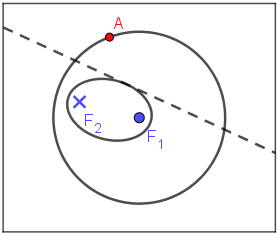
\includegraphics[width=0.3\textwidth]{images/stožnice/elipsa_dokaz1.png}
        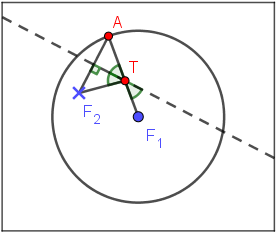
\includegraphics[width=0.3\textwidth]{images/stožnice/elipsa_dokaz2.png}
        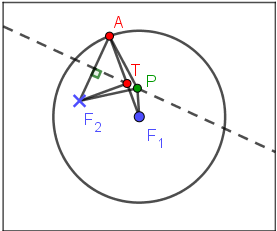
\includegraphics[width=0.3\textwidth]{images/stožnice/elipsa_dokaz3.png}
        \caption[Prepogibanje elipse]{Prepogibanje krožnice na izbrano točko znotraj nje.}
        \label{fig:dokaz_elipsa}
    \end{figure}  
\end{dokaz}

\textcolor{red}{še dokaz, da je OBRIS elipsa, kot prej s parabolo npr.\ iz kvadratne enačbe?}

Kaj pa, če pri konstrukciji izberemo točko izven krožnice?

\subsection{Hiperbola}

\textit{\textbf{Aktivnost:} Vzemi list papirja in svinčnik ter na sredini nariši poljubno krožnico. Označi njeno središče. Na zunanji strani krožnice si izberi poljubno točko. Izberi si točko na krožnici in list prepogni tako, da se obe izbrani točki prekrijeta. To ponovi čimvečkrat (gl.\ sliko~\ref{fig:koraki_elipsa}). Kaj opaziš?}

\subsection{Krožnica}

?